\section{Execution}

\subsection{Experimental setup}

The experiment consisted of a motor that was to control, a tachometer and a controller. To make things more exciting, the system also featured disturbances, emulated by a switch coupling in some resistors.

The setup can be seen in Figure \ref{fig:setup}. The block diagram characterizing the ytem is depicted in Figure \ref{fig:blockdiagram}.

\begin{figure}[H]
\begin{center}s
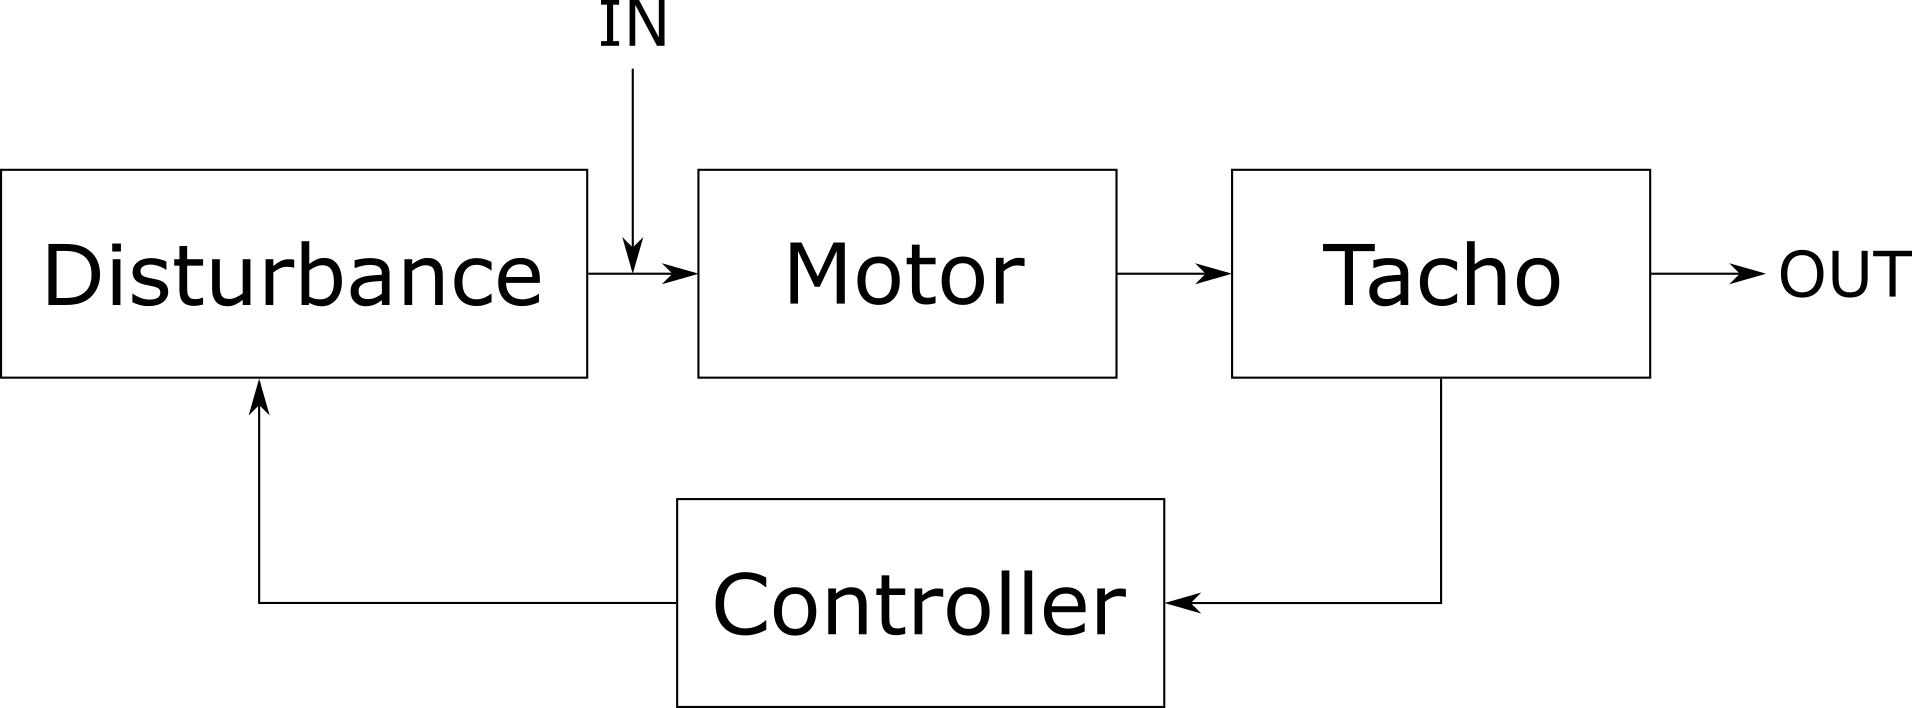
\includegraphics[width=0.6\linewidth]{images/general/motor_system}
\end{center}
\caption{Block diagram of the system}
\label{fig:blockdiagram}
\end{figure}

\subsection{Knowing the system}

At first the characteristic curve of the system was recorded to learn more about the limitations of the system. This was done by measuring the outputs for a broad range of inputs.

The highest possible input was 13 Volts whilst the lowest was -13 Volts. This resulted in aproximately 101 turns per minute in either clockwise or counter clockwise direction.
The characteristic curve is plotted in Figure \ref{fig:characteristic_curve}

Knowing the limits, an operating point of approcimately 7 Volts was chosen which results in around 50 turns. This operatng point as chosen since a system is hard to control at its boundaries. This value isn't to close to the upper limit and ensures that the controller has it's freedom.

Sadly a mistake was made  with the settings and all the experiments were done at an operating point of 90 turns per minute. So this should be kept in mind in the further reading.

\subsection{Carrying out the step experiment}

To properly implement a PID using the Chien Hrones Reswick method, the curve seen in Figure \ref{fig:step_experiment} was analyzed and the parameters in Table \ref{tab:step_params} were determined:

\begin{table}[H]
\begin{center}
\begin{tabular}{ l | r}
  Parameter & Value\\
  \hline
  \hline
  $K_s$ & $10$\\
  \hline
  $T_u$ & $1s$\\
  \hline
  $T_g$ & $2s$\\
  \hline
\end{tabular}
\end{center}
\caption{Chien, Hrones, Reswick Parameter}
\label{tab:step_params}
\end{table}

This was done using the approach of analyzing the step function of the system. This process is explained in Section \ref{subs:Chien, Hrones, Reswick}.

\subsection{Tinkering with the oscillation method}

Using the oscillation approach, the parameters listed in Table \ref{tab:osc_params} were determined.

\begin{table}[H]
\begin{center}
\begin{tabular}{ l | r}
  Parameter & Value\\
  \hline
  \hline
  $K_{P,crit}$ & $1.4$\\
  \hline
  $\tau_{crit}$ & $8/3s$\\
  \hline
\end{tabular}
\end{center}
\caption{Ziegler-Nichols Parameter}
\label{tab:osc_params}
\end{table}

Those parameters can be found by studying the curves seen in Figures \ref{fig:osc_experiment1} and \ref{fig:osc_experiment2} using the method explained in Section \ref{subs:Ziegler-Nichols}.